\documentclass[conference]{IEEEtran}
\usepackage{graphicx}
\usepackage{amsmath}
\usepackage{listings}
\usepackage{xcolor}
\usepackage{tikz}
\usetikzlibrary{shapes.geometric, arrows}

\lstset{
  basicstyle=\ttfamily\footnotesize,
  keywordstyle=\color{blue},
  commentstyle=\color{green},
  stringstyle=\color{red},
  numbers=left,
  numberstyle=\tiny\color{gray},
  stepnumber=1,
  numbersep=5pt,
  backgroundcolor=\color{lightgray},
  tabsize=2,
  showspaces=false,
  showstringspaces=false,
  breaklines=true
}

\begin{document}

\title{English Spell Correcting Chatbot using Natural Language Processing techniques}

\author{\IEEEauthorblockN{Sana Izumi}
\IEEEauthorblockA{University of San Carlos\\
Email: 20101443@usc.edu.ph}
}

\maketitle

\begin{abstract}
Brief summary of the project, objectives, and results.
\end{abstract}

\section{Introduction}
\medskip

\hspace{10pt}Natural Language Processing (NLP) is a branch of artificial intelligence (AI) utilized to analyze and interpret written and verbal human language. The primary objective is to design programs that can generate and comprehend natural language, enabling people to communicate with computers and have computers analyze their needs.\cite{NLPFrank} Machine learning is finding more and more applications in data analytics, such as the creation of chatbots that can mimic human user discussions by extracting relevant insights from massive databases. \cite{NLPFrank}

\medskip

\hspace{10pt}One prominent application of NLP is the development of chatbots. Chatbots utilize NLP to facilitate human-like interactions between computers and users, offering a wide range of functionalities from customer service to personal assistance. In this project, the primary function of the chatbot is spell correction. Spell correction tools are essential for enhancing written communication by automatically identifying and rectifying spelling errors. For non-native English learners, spell correction tools serve as a valuable aid, helping them to learn and use new vocabulary accurately. This chatbot will not only help users recognize and correct their spelling mistakes but also enhance their overall learning experience by reinforcing the correct spelling of words.

\medskip

\hspace{10pt}The primary objective of this project is to apply the concepts and techniques learned in NLP to develop a practical tool that assists non-native English learners in improving their vocabulary. This chatbot utilize various NLP concepts such as tokenization, vectorization, and neural networks to detect, correct spelling errors, and provide real-time feedback to users.

\section{Relevance/Significance}
\subsection{Importance of Spell Correction for Non-Native English Learners}
The ability to write correctly is fundamental to effective communication. For non-native English learners, mastering spelling is a crucial aspect of their language acquisition journey. Spell correction tools can significantly alleviate the challenges faced by these learners by providing immediate feedback and corrections. This not only helps in minimizing errors but also aids in reinforcing the correct spelling of words, thereby improving their overall proficiency in English.

Inaccurate spelling can lead to misunderstandings, reduced readability, and a lack of professionalism in written communication. In educational settings, spelling mistakes can hinder the learning process, causing confusion and impeding the acquisition of new vocabulary. Therefore, integrating effective spell correction capabilities into educational tools is vital for supporting learners in developing their language skills.

\subsection{Enhancing Digital Communication}
In the digital age, written communication is ubiquitous, spanning emails, text messages, social media posts, and more. Accurate spelling is essential for clear and professional communication. Spell correction tools embedded in chatbots can play a pivotal role in ensuring that users' written communication is free of errors. This is particularly relevant in professional and educational contexts, where precision in language is crucial.

\subsection{Advancements in NLP and Educational Technology}
The development of this spell-correcting chatbot exemplifies the practical application of advanced NLP techniques. By leveraging concepts such as tokenization, vectorization, and neural networks, this project showcases how theoretical knowledge can be transformed into a functional and beneficial tool. This not only underscores the versatility of NLP in solving real-world problems but also highlights its potential to revolutionize educational technology.

\section{Methodology}

\subsection{Flowchart of Methodology}
The following flowchart illustrates the steps involved in developing the spell-correcting chatbot:
\begin{figure}[h!]
    \centering
    \documentclass{standalone}
\usepackage{tikz}
\usetikzlibrary{shapes.geometric, arrows}

\tikzstyle{startstop} = [rectangle, rounded corners, minimum width=3cm, minimum height=1cm, text centered, draw=black, fill=red!30]
\tikzstyle{process} = [rectangle, minimum width=3cm, minimum height=1cm, text centered, draw=black, fill=orange!30]
\tikzstyle{arrow} = [thick,->,>=stealth]

\begin{document}

\begin{tikzpicture}[node distance=2cm]

\node (start) [startstop] {Start};
\node (collect) [process, below of=start] {Collect Dataset};
\node (introduce) [process, below of=collect] {Introduce Misspellings};
\node (combine) [process, below of=introduce] {Combine Correct and Misspelled Words};
\node (tokenize) [process, below of=combine] {Tokenize and Vectorize};
\node (split) [process, below of=tokenize] {Split Data into Training and Testing Sets};
\node (logreg) [process, below of=split] {Train Logistic Regression Model};
\node (lstm) [process, below of=logreg] {Train LSTM Model};
\node (evaluate) [process, below of=lstm] {Evaluate Models};
\node (chatbot) [process, below of=evaluate] {Implement Chatbot};
\node (end) [startstop, below of=chatbot] {End};

\draw [arrow] (start) -- (collect);
\draw [arrow] (collect) -- (introduce);
\draw [arrow] (introduce) -- (combine);
\draw [arrow] (combine) -- (tokenize);
\draw [arrow] (tokenize) -- (split);
\draw [arrow] (split) -- (logreg);
\draw [arrow] (logreg) -- (lstm);
\draw [arrow] (lstm) -- (evaluate);
\draw [arrow] (evaluate) -- (chatbot);
\draw [arrow] (chatbot) -- (end);

\end{tikzpicture}

\end{document}

    \caption{Flowchart of the methodology for developing the spell-correcting chatbot.}
    \label{fig:flowchart}
\end{figure}

\subsection{Data Collection and Preprocessing}
The first step in developing the spell-correcting chatbot was to collect and preprocess the data. I utilized the words corpus from the Natural Language Toolkit (NLTK), which contains a comprehensive list of English words. This dataset provided the foundation for both correctly spelled words and misspelled variants.

\subsubsection{Introducing Misspellings}
To simulate real-world scenarios where users may input misspelled words, I created a function to introduce random misspellings into the dataset. This function, introduce_misspellings, modifies a given word by randomly replacing one of its characters with another character from the alphabet, based on a specified error rate. The experimented error rates were 0.1(10\%), 0.5(50\%), and 0.8(80\%). This process generated a diverse set of misspelled words to train the model effectively.
\begin{lstlisting}[language=Python, caption=Data Collection and Preprocessing]
    import nltk
    from nltk.corpus import words
    import random
    
    # Download the dataset if not already done
    nltk.download('words')
    
    # Load the dataset
    word_list = words.words()
    
    # Function to introduce misspellings
    def introduce_misspellings(word, error_rate=0.1):
        if random.random() < error_rate:
            index = random.randint(0, len(word) - 1)
            return word[:index] + random.choice('abcdefghijklmnopqrstuvwxyz') + word[index + 1:]
        return word
    
    # Create a dataset with misspellings
    misspelled_word_list = [introduce_misspellings(word) for word in word_list]
    
\end{lstlisting}

\subsubsection{Combining Correct and Misspelled Words}
I combined the original correctly spelled words with the newly generated misspelled words to create a comprehensive dataset. Each word in the dataset was labeled as either correct (0) or misspelled (1).
\begin{lstlisting}[language=Python, caption=Data Collection and Preprocessing]
    # Combine correct and misspelled words
    combined_word_list = word_list + misspelled_word_list
    labels = [0] * len(word_list) + [1] * len(misspelled_word_list)    
\end{lstlisting}

\subsection{Tokenization and Vectorization}
To prepare the data for training, I used tokenization and vectorization techniques. Tokenization involved breaking down the words into individual characters, which were then converted into sequences of numerical values using the Keras Tokenizer. These sequences were padded to ensure uniform length, facilitating input into the neural network.

\subsection{Data Splitting}
The dataset was split into training and testing sets, with 80\% of the data used for training and 20\% reserved for testing. This ensured that the model was evaluated on data it had not seen during training, providing an accurate measure of its performance.

\subsection{Logistic Regression Model}
Initially, I implemented a Logistic Regression model with a pipeline using the 'liblinear' solver. This model served as a baseline to compare the performance with the more complex LSTM-based neural network.
\begin{lstlisting}[language=Python, caption=Data Collection and Preprocessing]
    from sklearn.preprocessing import StandardScaler
    from sklearn.pipeline import Pipeline
    from sklearn.model_selection import train_test_split
    from sklearn.linear_model import LogisticRegression
    from sklearn.metrics import accuracy_score, classification_report
    
    # Split the data
    X_train, X_test, y_train, y_test = train_test_split(X, labels, test_size=0.2, random_state=42)
    
    # Create a pipeline with scaling and logistic regression using 'liblinear' solver
    pipeline = Pipeline([
        ('scaler', StandardScaler(with_mean=False)),  # Scaling the data
        ('logreg', LogisticRegression(max_iter=1000, solver='liblinear'))  # Use 'liblinear' solver
    ])
    
    # Train the model
    pipeline.fit(X_train, y_train)
    
    # Evaluate the model
    y_pred = pipeline.predict(X_test)
    print(f"Accuracy: {accuracy_score(y_test, y_pred)}")
    print(classification_report(y_test, y_pred))
\end{lstlisting}


\subsection{LSTM-Based Neural Network Model}
To optimize and improve the accuracy, I built an LSTM-based neural network model according to Dhankhar(2018)\cite{DhanLSTM}. The model architecture consisted of an embedding layer, two LSTM layers, and a dense output layer with a sigmoid activation function.

¥begin{itemize}
    ¥item Embedding Layer: Converts the input sequences into dense vectors of fixed size.
    ¥item LSTM Layers: Capture the sequential dependencies in the character sequences.
    ¥item Dense Output Layer: Provides a binary classification output (correct or misspelled).
¥end{itemize}

\begin{lstlisting}[language=Python, caption=Data Collection and Preprocessing]
    from keras.models import Sequential
    from keras.layers import Embedding, LSTM, Dense
    
    # Build LSTM model
    model = Sequential()
    model.add(Embedding(input_dim=len(tokenizer.word_index) + 1, output_dim=50, input_length=max_seq_length))
    model.add(LSTM(100, return_sequences=True))
    model.add(LSTM(100))
    model.add(Dense(1, activation='sigmoid'))
    
    # Compile the model
    model.compile(optimizer='adam', loss='binary_crossentropy', metrics=['accuracy'])
    
\end{lstlisting}

\subsection{Training and Evaluation}
I experimented and turned with different hyperparameters, such as the error rate for generating misspellings, the number of epochs, and the batch size, to find the optimal configuration for the LSTM model. The final model was trained for 10 epochs with a batch size of 64 using error rate 0.8(80\%). The validation dataset was used to monitor the model's performance during training. After training, the model's accuracy was evaluated on the test dataset.
\begin{lstlisting}[language=Python, caption=Data Collection and Preprocessing]
    # Train the model
    history = model.fit(X_train, y_train, epochs=10, batch_size=64, validation_data=(X_test, y_test))
    
    # Evaluate the model
    loss, accuracy = model.evaluate(X_test, y_test)
    print(f"LSTM Model Accuracy: {accuracy}")
    
    # Predict and evaluate
    y_pred = (model.predict(X_test) > 0.5).astype("int32")
    print(f"LSTM Model Accuracy: {accuracy_score(y_test, y_pred)}")
    print(classification_report(y_test, y_pred))
    
\end{lstlisting}

\subsection{Chatbot Implementation}
The chatbot function was designed to take user input, preprocess it, and use the trained model to predict whether the input word was correctly spelled or not. If the word is misspelled, the chatbot suggest the most similar correctly spelled word based on character similarity and also displayed its matching accuracy. If the word is spelled correctly, the chatbot return "Nothing Wrong!".
\begin{lstlisting}[language=Python, caption=Data Collection and Preprocessing]
    # Chatbot function to correct spelling
    def correct_spelling(input_word):
        input_seq = tokenizer.texts_to_sequences([input_word])
        input_seq = pad_sequences(input_seq, maxlen=max_seq_length)
        
        prediction = model.predict(input_seq)
        
        if prediction < 0.5:
            return "Nothing Wrong!"
        
        # Find the most similar word
        similarities = []
        for word in word_list:
            if len(word) == len(input_word):
                sim = sum(1 for a, b in zip(word, input_word) if a == b)
                similarities.append((word, sim))
        if not similarities:
            return "No suggestions available."
        
        best_match = max(similarities, key=lambda x: x[1])[0]
        accuracy = max(similarities, key=lambda x: x[1])[1] / len(input_word) * 100
        
        return f"Suggested Correction: {best_match}, Matching Accuracy: {accuracy:.2f}%"
    
    # Simple chatbot interface
    def chatbot():
        print("Welcome to the English Correcting Chatbot! Type 'exit' to quit.")
        while True:
            user_input = input("Enter a word: ").strip()
            if user_input.lower() == 'exit':
                break
            correction = correct_spelling(user_input)
            print(correction)
    
    # Run the chatbot
    chatbot()
    
\end{lstlisting}



\section{Results and Analysis}
This section provides a comprehensive overview of the evaluation criteria, results, and analysis for both the Logistic Regression and LSTM-based neural network models, along with observations from the chatbot usage. By detailing the different conditions and their corresponding metrics, the analysis highlights the improvements achieved with the LSTM model and provides insights into the model's performance under various configurations.

\subsection{Evaluation Criteria}
Based on the study by Katsumata(2020)\cite{Katsumata}, I used these metrics to evaluate the performance of the spell-correcting chatbot:
\begin{itemize}
    \item \textbf{Accuracy}: The proportion of correctly identified instances (correct or misspelled) out of the total instances.
    \item \textbf{Precision}: The ratio of correctly predicted positive observations to the total predicted positives.
    \item \textbf{Recall}: The ratio of correctly predicted positive observations to all observations in the actual class.
    \item \textbf{F1 Score}: The weighted average of Precision and Recall, providing a balance between the two.
\end{itemize}

These metrics provide a comprehensive evaluation of the models' performance, considering both their ability to correctly identify misspellings and their reliability in predicting the correct class.

\subsection{Logistic Regression Model}

I experimented with the Logistic Regression model using three different error rates for introducing misspellings: 10\%, 50\%, and 80\%. Regardless of the error rate, the results were consistent across all trials.

\subsubsection{Logistic Regression Model Results}

\begin{verbatim}
Accuracy: 0.4645
              precision    recall  f1-score   support

           0       0.47      0.65      0.55     47305
           1       0.44      0.28      0.35     47390

    accuracy                           0.46     94695
   macro avg       0.46      0.46      0.45     94695
weighted avg       0.46      0.46      0.45     94695
\end{verbatim}

\begin{figure}[h!]
    \centering
    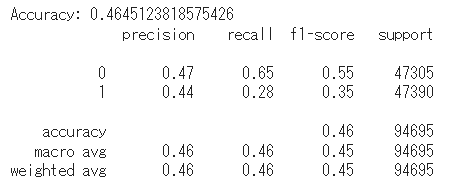
\includegraphics[width=0.3\textwidth]{LogiReg_result.png}
    \caption{Evaluation results of Logistic Regression model.}
    \label{fig:logreg_results}
\end{figure}

\subsection{LSTM-Based Neural Network Model}

To optimize and improve accuracy, I built an LSTM-based neural network model. I experimented with various combinations of error rates, epochs, and batch sizes:

\begin{itemize}
    \item \textbf{(error rate = 0.1, epochs = 10, batch size = 64)}
    \item \textbf{(error rate = 0.5, epochs = 10, batch size = 64)}
    \item \textbf{(error rate = 0.5, epochs = 10, batch size = 32)}
    \item \textbf{(error rate = 0.8, epochs = 10, batch size = 64)}
\end{itemize}

\subsubsection{LSTM Model Results}

1. \textbf{(error rate = 0.1, epochs = 10, batch size = 64)}
\begin{verbatim}
Accuracy: 0.5153
              precision    recall  f1-score   support

           0       0.51      0.76      0.61     47305
           1       0.53      0.27      0.36     47390

    accuracy                           0.52     94695
   macro avg       0.52      0.52      0.48     94695
weighted avg       0.52      0.52      0.48     94695
\end{verbatim}

\begin{figure}[h!]
    \centering
    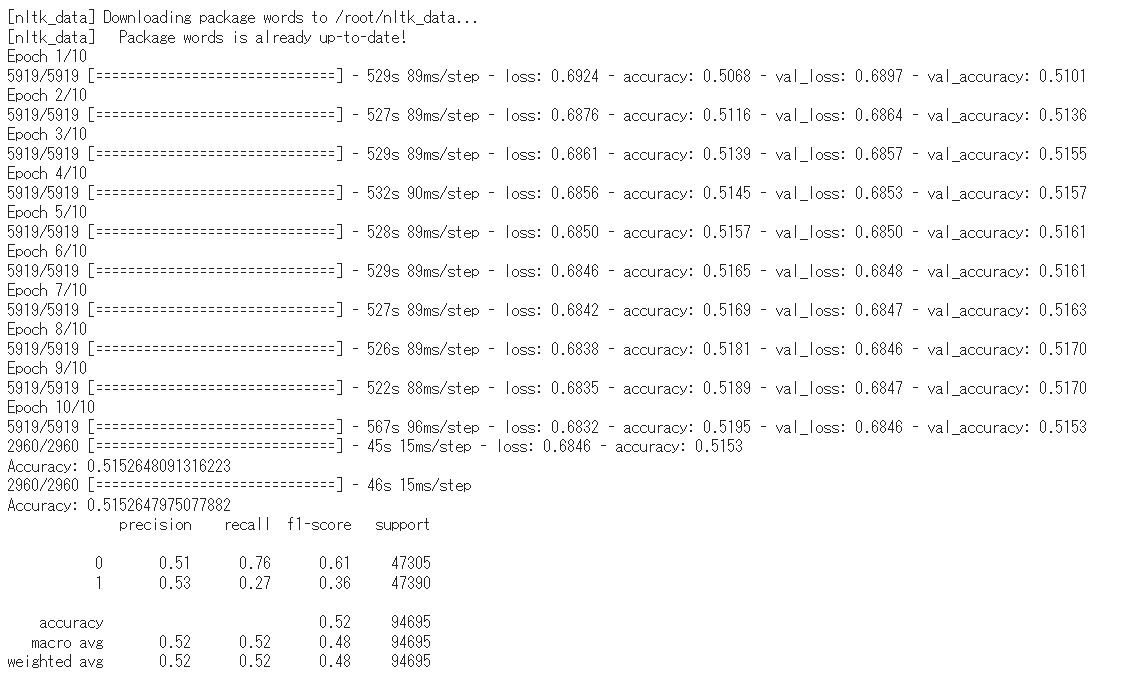
\includegraphics[width=0.3\textwidth]{ER10_epoch10_batch64.png}
    \caption{Evaluation results of LSTM model with error rate 0.1, epochs 10, batch size 64.}
    \label{fig:lstm_results_0.1_10_64}
\end{figure}

2. \textbf{(error rate = 0.5, epochs = 10, batch size = 64)}
\begin{verbatim}
Accuracy: 0.6380
              precision    recall  f1-score   support

           0       0.59      0.91      0.71     47305
           1       0.80      0.37      0.50     47390

    accuracy                           0.64     94695
   macro avg       0.69      0.64      0.61     94695
weighted avg       0.69      0.64      0.61     94695
\end{verbatim}

\begin{figure}[h!]
    \centering
    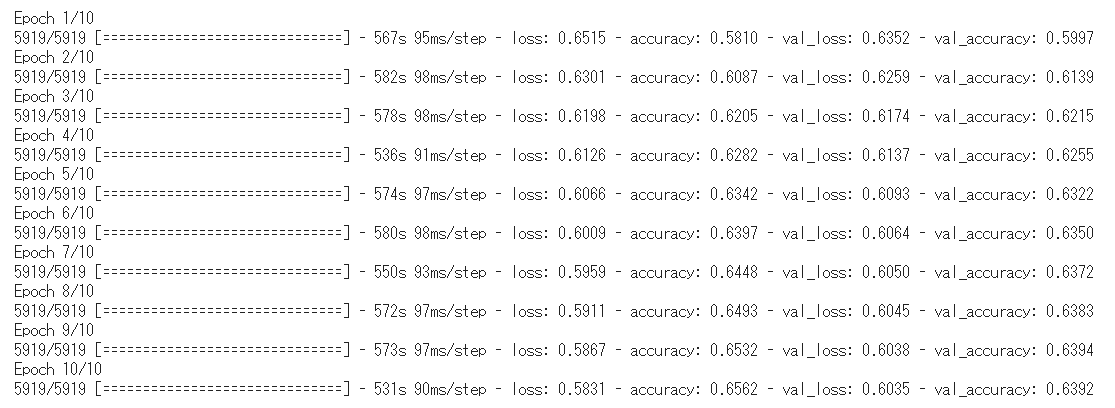
\includegraphics[width=0.3\textwidth]{1-ER50_epoch10_batch64.png}
    \label{fig:lstm_results_0.5_10_64-1}
\end{figure}
\begin{figure}[h!]
    \centering
    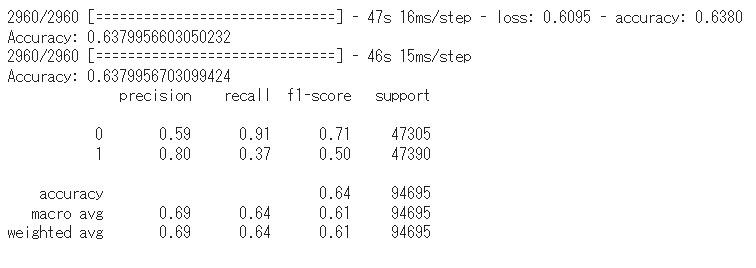
\includegraphics[width=0.3\textwidth]{2-ER50_epoch10_batch64.png}
    \caption{Evaluation results of LSTM model with error rate 0.5, epochs 10, batch size 64.}
    \label{fig:lstm_results_0.5_10_64-2}
\end{figure}

3. \textbf{(error rate = 0.5, epochs = 10, batch size = 32)}
\begin{verbatim}
Accuracy: 0.6408
              precision    recall  f1-score   support

           0       0.59      0.91      0.72     47305
           1       0.81      0.37      0.51     47390

    accuracy                           0.64     94695
   macro avg       0.70      0.64      0.61     94695
weighted avg       0.70      0.64      0.61     94695
\end{verbatim}

\begin{figure}[h!]
    \centering
    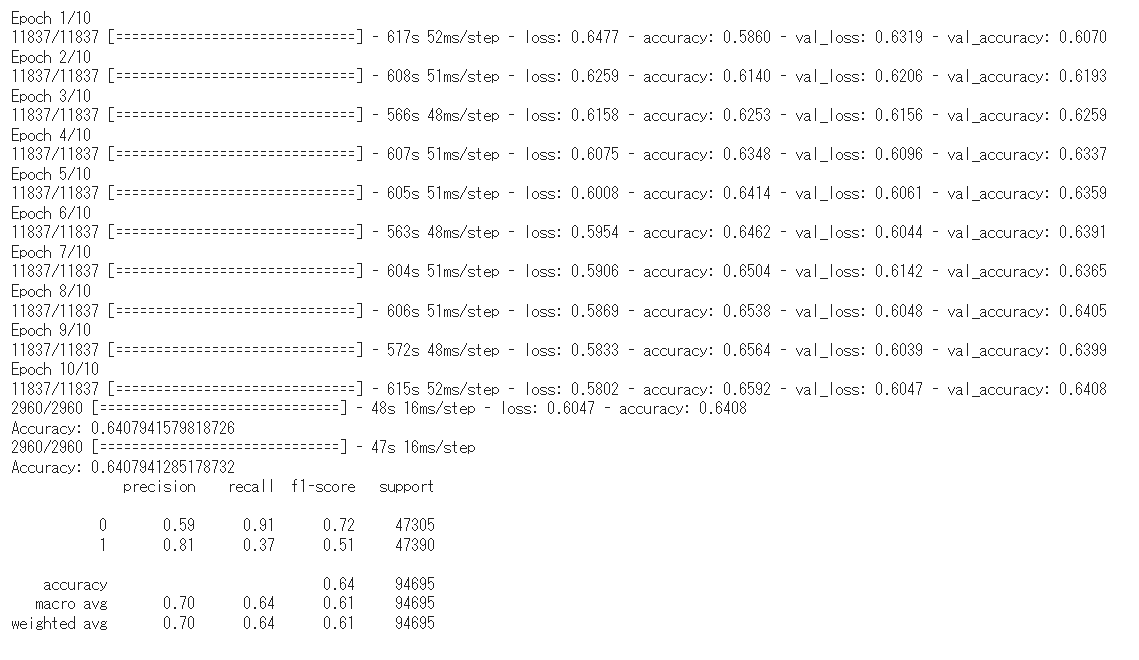
\includegraphics[width=0.3\textwidth]{ER50_epoch10_batch32.png}
    \caption{Evaluation results of LSTM model with error rate 0.5, epochs 10, batch size 32.}
    \label{fig:lstm_results_0.5_10_32}
\end{figure}

4. \textbf{(error rate = 0.8, epochs = 10, batch size = 64)}
\begin{verbatim}
Accuracy: 0.7451
              precision    recall  f1-score   support

           0       0.69      0.89      0.78     47305
           1       0.84      0.60      0.70     47390

    accuracy                           0.75     94695
   macro avg       0.77      0.75      0.74     94695
weighted avg       0.77      0.75      0.74     94695
\end{verbatim}

\begin{figure}[h!]
    \centering
    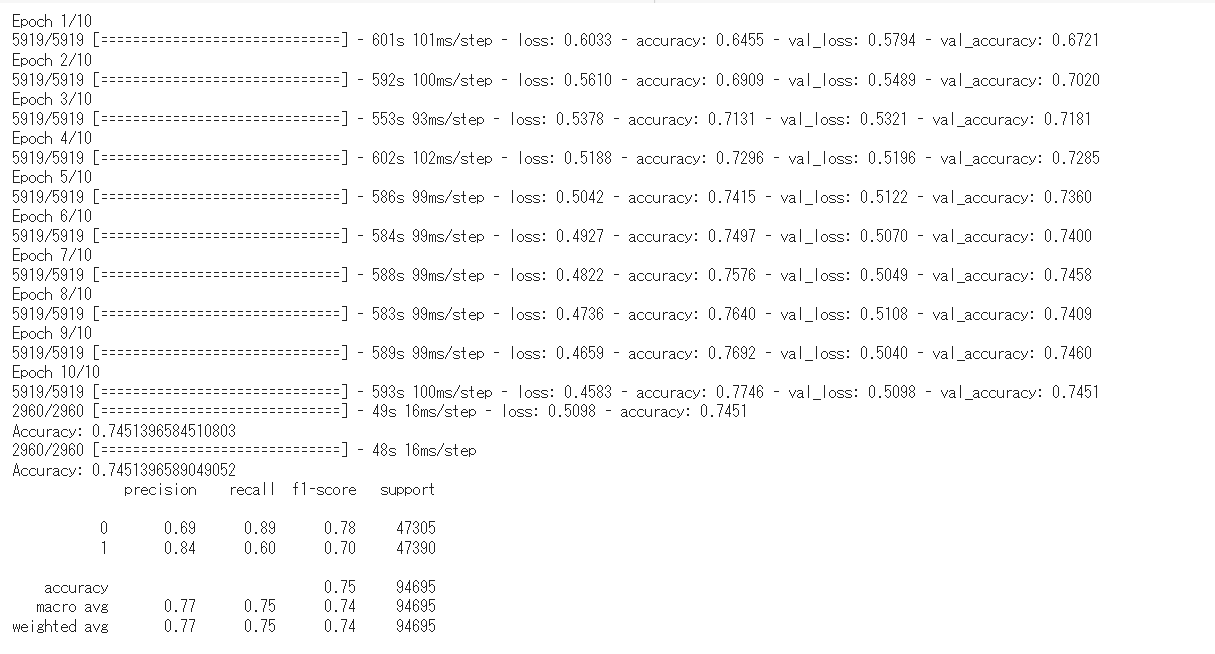
\includegraphics[width=0.3\textwidth]{ER80_epoch10_batch64.png}
    \caption{Evaluation results of LSTM model with error rate 0.8, epochs 10, batch size 64.}
    \label{fig:lstm_results_0.8_10_64}
\end{figure}

\subsection{Analysis}

\subsubsection{Logistic Regression Model}

The Logistic Regression model achieved an accuracy of approximately 46.45\%, with a precision of 0.47 for class 0 (correct words) and 0.44 for class 1 (misspelled words). The recall for class 0 was higher (0.65) compared to class 1 (0.28), indicating that the model was better at identifying correctly spelled words than misspelled ones. The F1 score, a balance between precision and recall, was moderate for class 0 (0.55) and lower for class 1 (0.35).

Overall, the Logistic Regression model provided a baseline performance but lacked the capability to accurately detect and correct misspelled words, regardless of the error rate used.

\subsubsection{LSTM-Based Neural Network Model}

The LSTM model showed significant improvement over the Logistic Regression model, with varying results based on the error rate and batch size:

1. \textbf{(error rate = 0.1, epochs = 10, batch size = 64)}: Accuracy was 51.53\%, with better performance for class 0 (precision: 0.51, recall: 0.76) compared to class 1 (precision: 0.53, recall: 0.27).

2. \textbf{(error rate = 0.5, epochs = 10, batch size = 64)}: Accuracy increased to 63.80\%, with notable improvements in class 1 detection (precision: 0.80, recall: 0.37).

3. \textbf{(error rate = 0.5, epochs = 10, batch size = 32)}: Slightly better accuracy at 64.08\%, with similar performance metrics as the previous configuration.

4. \textbf{(error rate = 0.8, epochs = 10, batch size = 64)}: The highest accuracy achieved was 74.51\%, with significant improvements in both precision and recall for class 1 (precision: 0.84, recall: 0.60).

These results indicate that the LSTM model is more effective at handling higher error rates, showing robust performance in detecting and correcting misspelled words. The choice of batch size also played a role, with smaller batch sizes slightly improving accuracy and F1 scores.

\subsection{Observations from Chatbot Usage}

Despite the improved metrics with the LSTM model, the real-world usage of the chatbot revealed that the suggestion accuracy was quite low. This discrepancy highlights a common challenge in NLP and machine learning: metrics may not fully capture the practical effectiveness of a model. User experience can often expose limitations that quantitative evaluations might overlook.

\begin{figure}[h!]
    \centering
    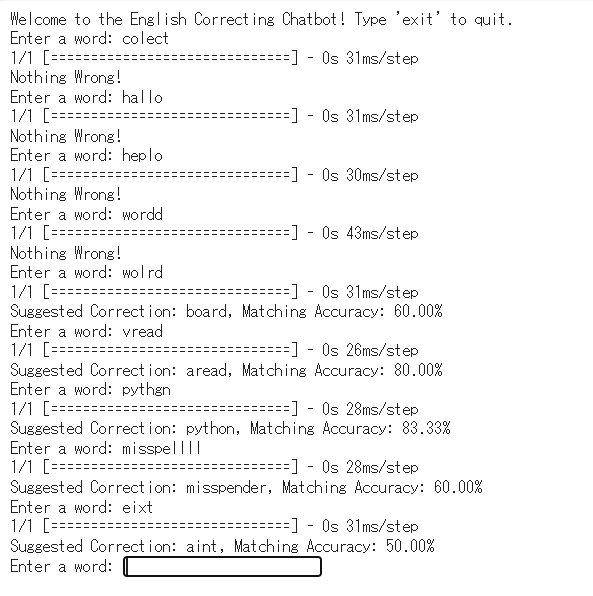
\includegraphics[width=0.3\textwidth]{chatbot_display.png}
    \caption{Example Chatbot Usage.}
    \label{fig:lchatbot_display}
\end{figure}

\section{Conclusion}
This project demonstrated the application of Natural Language Processing (NLP) techniques to develop a spell-correcting chatbot aimed at assisting non-native English learners in improving their vocabulary and writing skills. The primary focus was on implementing and comparing two models: a Logistic Regression model and an LSTM-based neural network model. While the LSTM model showed significant improvements over the Logistic Regression model in terms of accuracy, precision, recall, and F1 score, practical usage of the chatbot indicated that suggestion accuracy needs further improvement. Future work could focus on incorporating ither different neural network architectures and introducing different mechanisms to generate and compare the misspelled words dataset, to enhance the model accuracy.


\bibliographystyle{IEEEtran}
\bibliography{References}

\end{document}
